\documentclass[paper=a4, fontsize=11pt]{scrartcl} 

\usepackage[T1]{fontenc} 
\usepackage[english]{babel}
\usepackage{amsmath,amsfonts,amsthm}

\usepackage{lipsum}

\usepackage{graphicx}
\usepackage{float}
  \floatplacement{figure}{H}
  \floatplacement{table}{H}
  
\usepackage{sectsty} 
\allsectionsfont{\centering \normalfont\scshape} 

\usepackage{fancyhdr} % Custom headers and footers
\pagestyle{fancyplain} % Makes all pages in the document conform to the custom headers and footers
\fancyhead{} % No page header - if you want one, create it in the same way as the footers below
\fancyfoot[L]{} % Empty left footer
\fancyfoot[C]{} % Empty center footer
\fancyfoot[R]{\thepage} % Page numbering for right footer
\renewcommand{\headrulewidth}{0pt} % Remove header underlines
\renewcommand{\footrulewidth}{0pt} % Remove footer underlines
\setlength{\headheight}{13.6pt} % Customize the height of the header

\usepackage[labelformat=empty]{caption}
\usepackage{color}
\usepackage{listings}
\lstset{ %
language=bash,                % choose the language of the code
basicstyle=\footnotesize,       % the size of the fonts that are used for the code
numbers=left,                   % where to put the line-numbers
numberstyle=\footnotesize,      % the size of the fonts that are used for the line-numbers
stepnumber=1,                   % the step between two line-numbers. If it is 1 each line will be numbered
numbersep=5pt,                  % how far the line-numbers are from the code
backgroundcolor=\color{white},  % choose the background color. You must add \usepackage{color}
showspaces=false,               % show spaces adding particular underscores
showstringspaces=false,         % underline spaces within strings
showtabs=false,                 % show tabs within strings adding particular underscores
frame=single,           % adds a frame around the code
tabsize=2,          % sets default tabsize to 2 spaces
captionpos=b,           % sets the caption-position to bottom
breaklines=true,        % sets automatic line breaking
breakatwhitespace=false,    % sets if automatic breaks should only happen at whitespace
escapeinside={\%*}{*)}          % if you want to add a comment within your code
}
\usepackage{hyperref}


\numberwithin{equation}{section} % Number equations within sections (i.e. 1.1, 1.2, 2.1, 2.2 instead of 1, 2, 3, 4)
\numberwithin{figure}{section} % Number figures within sections (i.e. 1.1, 1.2, 2.1, 2.2 instead of 1, 2, 3, 4)
\numberwithin{table}{section} % Number tables within sections (i.e. 1.1, 1.2, 2.1, 2.2 instead of 1, 2, 3, 4)

\setlength\parindent{0pt} % Removes all indentation from paragraphs - comment this line for an assignment with lots of text

%----------------------------------------------------------------------------------------
%	TITLE SECTION
%----------------------------------------------------------------------------------------

\newcommand{\horrule}[1]{\rule{\linewidth}{#1}} % Create horizontal rule command with 1 argument of height

\title{	
\normalfont \normalsize 
\textsc{Computational Science} \\ [25pt] % Your university, school and/or department name(s)
\horrule{0.5pt} \\[0.2cm] % Thin top horizontal rule
\small Homework - Introduction to Frontiers of Computational Science\\ % The assignment title
%\horrule{2pt} \\[0.5cm] % Thick bottom horizontal rule
}

\author{\small{Ridlo W. Wibowo || 1215011069}} % Your name

\date{\small\today} % Today's date or a custom date


\begin{document}
\maketitle % Print the title

\textbf{Problem 1.}\\
In a fluid we can define a fluid parcel, a very small amount of fluid which is moving with the fluid flow.\\
\begin{figure}
	\centering
	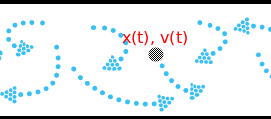
\includegraphics[width=0.3\textwidth]{fluid_flow.png}
	\caption{Fluid parcel moving around with a flow velocity $\textbf{v}(\textbf{x},t)$ at position $\textbf{X}(t)$.}
\end{figure}

Flow velocity at $\textbf{X} (x(t), y(t), z(t))$ at time $t$ is described by a function:\\
\begin{equation*}
\textbf{v}(\textbf{X}(t), t) = \frac{\partial \textbf{X}(t)}{\partial t} 
\end{equation*}

and the temperature of fluid at position $\textbf{X}$ is described by a function $\theta = \Theta(\textbf{X},t)$

Prove:
\begin{equation*}
\frac{D\theta}{Dt} = \frac{\partial \Theta}{\partial t} + \textbf{v} \cdot \nabla \Theta
\end{equation*}

Using chain rule:
\begin{eqnarray*}
\frac{D\theta}{Dt} & = & \frac{D \Theta(\textbf{X},t)}{Dt}\\
 & = & \frac{\partial \Theta}{\partial t} + \frac{\partial \Theta}{\partial x} \frac{d x}{d t} + \frac{\partial \Theta}{\partial y} \frac{d y}{d t} + \frac{\partial \Theta}{\partial z} \frac{d z}{d t}\\
 & = & \frac{\partial \Theta}{\partial t} + (\textbf{v} \cdot \nabla) \Theta
\end{eqnarray*}

with $\textbf{v} = (\frac{dx}{dt}, \frac{dy}{dt}, \frac{dz}{dt})$ and $\nabla = (\frac{\partial }{\partial x}, \frac{\partial }{\partial y}, \frac{\partial }{\partial z})$.

\textbf{Problem 2.}\\
Solve this equation using Euler method:
\begin{equation*}
\frac{dx}{dt} = -\lambda x
\end{equation*}
with initial condition $x(0) = 1$ and $\lambda = 100$, find $x(1)$! Try different $\Delta t$ ($0.03$, $0.01$, and $0.001$).

Using Euler method means that we can solve this by:
\begin{eqnarray*}
x(t+\Delta t) &=& x(t) - \lambda x(t) \Delta t\\
&=& (1 - \lambda \Delta t) x(t)
\end{eqnarray*}
and the exact solution for this differential equation is $x(t) = e^{-\lambda t}$, so $x(1)$ should be $3.720076 \times 10^{-44}$.

Result:
\begin{table}[ht]
\begin{tabular}{c c}
\hline
$\Delta t$ & $x(1)$ \\ [0.5ex]
\hline 
0.1 & 3.48678e+09 \\
0.03 & -8.58993e+09 \\
0.01 & 0 \\
0.005 & 6.22302e-61 \\
0.001 & 1.74787e-46 \\
0.0001 & 2.24877e-44 \\ [1ex]
\hline 
\end{tabular}
\end{table}

Euler method is numerically unstable (conditionally stable) especially for stiff equations. Stable condition if $\vert z + 1 \vert \leq 1$, with $z = -\lambda dt$ for above equation. 
\begin{figure}
	\centering
	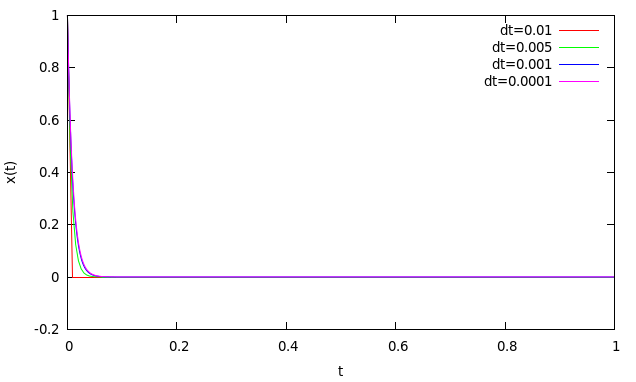
\includegraphics[width=0.49\textwidth]{euler1.png}
	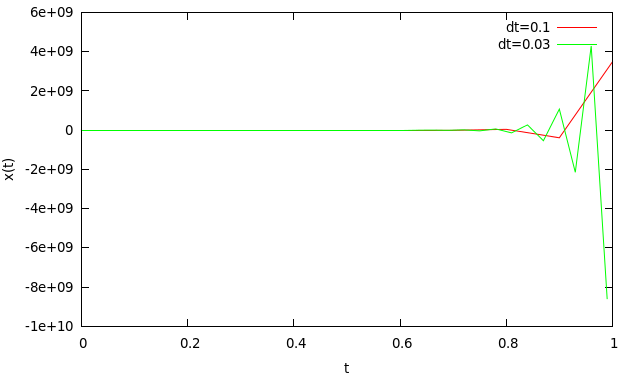
\includegraphics[width=0.49\textwidth]{euler2.png}
\end{figure}

\newpage
\textit{\textbf{Program}}
\lstset{frameround=fttt}
\begin{lstlisting}
#include <iostream>
#include <stdlib.h>
#include <math.h>
#include <fstream>
using namespace std;

void plot();
int main(int argc, char * argv[]){
    double lambda = 100., x0 = 1.;
    double ti = 0., tf = 1.;
    double dt = 0.001, x = x0, t = ti;
    
    if (argc <= 1){
        printf("Usage: %s dt\n", argv[0]);
    }
    if (argc > 1){
        dt = atof(argv[1]);
    }
         
    double N = (tf - ti)/dt;
    ofstream out("output.txt");
    out << t << " " << x << endl;
    for (int i=1;i<=N;i++){
        x = (1. - lambda*dt)*x;
        t = t+dt;
        out << t << " " << x << endl;
    }
    out.close();
    cout << "Exact value x(1) = 3.720076e-44\n"; 
    cout << "x(" << tf << ") = " << x << endl;
   
    plot();
    return 0;
}

void plot(){
    ofstream ploter("inp.plt");
    ploter << "#gnuplot input file\n";
    ploter << "set term png size 600,400\n";
    ploter << "set output \"euler.png\"\n";
    ploter << "set xlabel \"t\"\n";
    ploter << "set ylabel \"x(t)\"\n";
    ploter << "plot \"output.txt\" u 1:2 w l t \"x(t)\"\n";
    ploter.close();

    system("gnuplot inp.plt");
    system("rm inp.plt");
}
\end{lstlisting}

\end{document}